\documentclass{ximera}

%% You can put user macros here
%% However, you cannot make new environments

\listfiles

\graphicspath{{./}{firstExample/}{secondExample/}}

\usepackage{tikz}
\usepackage{tkz-euclide}
\usepackage{tikz-3dplot}
\usepackage{tikz-cd}
\usetikzlibrary{shapes.geometric}
\usetikzlibrary{arrows}
\usetikzlibrary{decorations.pathmorphing,patterns}
\usetkzobj{all}
\pgfplotsset{compat=1.13} % prevents compile error.

\renewcommand{\vec}[1]{\mathbf{#1}}
\newcommand{\RR}{\mathbb{R}}
\newcommand{\dfn}{\textit}
\newcommand{\dotp}{\cdot}
\newcommand{\id}{\text{id}}
\newcommand\norm[1]{\left\lVert#1\right\rVert}
 
\newtheorem{general}{Generalization}
\newtheorem{initprob}{Exploration Problem}

\tikzstyle geometryDiagrams=[ultra thick,color=blue!50!black]

\usepackage{mathtools}

\title{Constant Coefficient Homogeneous Systems III}%\label{Module 7-ADEF}


\begin{document}

\begin{abstract}

\end{abstract}

\maketitle

\section*{Constant Coefficient Homogeneous Systems III}

We now consider the system ${\bf y}'=A{\bf y}$, where $A$ has a complex
eigenvalue $\lambda=\alpha+i\beta$ with $\beta\ne0$. We continue to
assume that $A$ has real entries, so the characteristic polynomial of
$A$ has real coefficients. This implies that
$\overline\lambda=\alpha-i\beta$ is also an eigenvalue of $A$.

An eigenvector ${\bf x}$ of $A$ associated with
$\lambda=\alpha+i\beta$ will have complex entries, so we'll write
$$
{\bf x}={\bf u}+i{\bf v}
$$
where ${\bf u}$ and ${\bf v}$ have real entries; that is, ${\bf u}$
and ${\bf v}$ are the real and imaginary parts of ${\bf x}$. Since
$A{\bf x}=\lambda {\bf x}$,
\begin{equation} \label{eq:10.6.1}
A({\bf u}+i{\bf v})=(\alpha+i\beta)({\bf u}+i{\bf v}).
\end{equation}
Taking complex conjugates here and recalling that $A$ has real entries
yields
$$
A({\bf u}-i{\bf v})=(\alpha-i\beta)({\bf u}-i{\bf v}),
$$
which shows that ${\bf x}={\bf u}-i{\bf v}$ is an eigenvector
associated with $\overline{\lambda}=\alpha-i\beta$. The complex
conjugate eigenvalues $\lambda$ and $\overline{\lambda}$ can be
separately associated with linearly independent solutions ${\bf
y}'=A{\bf y}$;     however, we won't pursue this approach, since solutions
obtained in this way turn out to be complex--valued. Instead, we'll
obtain solutions of ${\bf y}'=A{\bf y}$ in the form
\begin{equation} \label{eq:10.6.2}
{\bf y}=f_1{\bf u}+f_2{\bf v}
\end{equation}
where $f_1$ and $f_2$ are real--valued scalar functions.
The next theorem shows how to do this.
% Changed by Felipe
\begin{theorem}\label{thmtype:10.6.1}
Let $A$ be an $n\times n$ matrix with real entries$.$ Let
$\lambda=\alpha+i\beta$ ($\beta\neq 0$) be a complex
eigenvalue of $A$ and let ${\bf x}={\bf u}+i{\bf v}$ be an associated
eigenvector$,$ where ${\bf u}$ and ${\bf v}$ have real components$.$ Then
${\bf u}$ and ${\bf v}$ are both nonzero and
$$
{\bf y}_1=e^{\alpha t}({\bf u}\cos\beta t-{\bf v}\sin\beta t)
\quad\mbox{and}\quad
{\bf y}_2=e^{\alpha t}({\bf u}\sin\beta t+{\bf v}\cos\beta t),
$$
which are the real and imaginary parts of
\begin{equation} \label{eq:10.6.3}
e^{\alpha t}(\cos\beta t+i\sin\beta t)({\bf u}+i{\bf v}),
\end{equation}
are linearly independent solutions of  ${\bf y}'=A{\bf y}$.
\end{theorem}

% Felipe added: \begin{proof}...\end{proof}
\begin{proof}
A function of the form \eqref{eq:10.6.2} is a solution of ${\bf y}'=A{\bf
y}$ if and only if
\begin{equation} \label{eq:10.6.4}
f_1'{\bf u}+f_2'{\bf
v}=f_1A{\bf u}+f_2A{\bf v}.
\end{equation}
Carrying out the multiplication indicated on the  right side
of \eqref{eq:10.6.1} and collecting the  real and imaginary parts of the
result yields
$$
A({\bf u}+i{\bf v})=(\alpha{\bf u}-\beta{\bf v})+i(\alpha{\bf v}+\beta{\bf
u}).
$$
Equating real and imaginary parts on the two sides of this equation yields
$$
\begin{array}{rcl}
A{\bf u}&=&\alpha{\bf u}-\beta{\bf v}\\
A{\bf v}&=&\alpha{\bf v}+\beta{\bf u}.
\end{array}
$$
\end{proof}
We leave it to you %(Exercise~\ref{exer:10.6.25}) 
to show from this that
${\bf u}$ and
${\bf v}$ are both nonzero.
Substituting from these equations into \eqref{eq:10.6.4} yields
\begin{eqnarray*}
f_1'{\bf u}+f_2'{\bf v}
&=&f_1(\alpha{\bf u}-\beta{\bf v})+f_2(\alpha{\bf v}+\beta{\bf u})\\
&=&(\alpha f_1+\beta f_2){\bf u}+(-\beta f_1+\alpha f_2){\bf v}.
\end{eqnarray*}
This is true if
$$
\begin{array}{rcr}
f_1'&=&\alpha f_1+\beta f_2\\
f_2'&=&-\beta f_1+\alpha f_2,
\end{array}
\quad\mbox{or, equivalently}\quad
\begin{array}{rcr}
f_1'-\alpha f_1&=&\beta f_2\\
f_2'-\alpha f_2&=&-\beta f_1.
\end{array}
$$
If we let $f_1=g_1e^{\alpha t}$ and $f_2=g_2e^{\alpha t}$, where
$g_1$ and $g_2$ are to be determined, then the last two equations
become
$$
\begin{array}{rcr}
g_1'&=&\beta g_2\\
g_2'&=&-\beta g_1,
\end{array}
$$
which implies that
$$
g_1''=\beta g_2'=-\beta^2 g_1,
$$
so
$$
g_1''+\beta^2 g_1=0.
$$
The general solution of this equation is
$$
g_1=c_1\cos\beta t+c_2\sin\beta t.
$$
Moreover, since $g_2=g_1'/\beta$,
$$
g_2=-c_1\sin\beta t+c_2\cos\beta t.
$$
Multiplying  $g_1$  and $g_2$  by $e^{\alpha t}$ shows that
\begin{eqnarray*}
f_1&=&e^{\alpha t}(c_1\cos\beta t+c_2\sin\beta t ),\\
f_2&=&e^{\alpha t}(-c_1\sin\beta t+c_2\cos\beta t).
\end{eqnarray*}
Substituting these into \eqref{eq:10.6.2} shows that
\begin{equation} \label{eq:10.6.5}
\begin{array}{rcl}
{\bf y}&=&e^{\alpha t}\left[(c_1\cos\beta t+c_2\sin\beta t){\bf u}
+(-c_1\sin\beta t+c_2\cos\beta t){\bf v}\right]\\
&=&c_1e^{\alpha t}({\bf u}\cos\beta t-{\bf v}\sin\beta t)
+c_2e^{\alpha t}({\bf u}\sin\beta t+{\bf v}\cos\beta t)
\end{array}
\end{equation}
is a solution of ${\bf y}'=A{\bf y}$ for any choice of the constants
$c_1$ and $c_2$. In particular, by first taking $c_1=1$ and $c_2=0$
and then taking $c_1=0$ and $c_2=1$, we see that ${\bf y}_1$ and ${\bf
y}_2$ are solutions of $ {\bf y}'=A{\bf y}$. We leave it to you to
verify that they are, respectively, the real and imaginary parts of
\eqref{eq:10.6.3}, %(Exercise~\ref{exer:10.6.26}), 
and that they are linearly
independent. %(Exercise~\ref{exer:10.6.27}).

\begin{example}\label{example:10.6.1}
 Find the general solution of
\begin{equation} \label{eq:10.6.6}
{\bf y}'=\begin{bmatrix}4&-5\\5&-2\end{bmatrix}{\bf y}.
\end{equation}

\begin{explanation} The characteristic polynomial of the coefficient matrix $A$
in \eqref{eq:10.6.6} is
$$
\begin{vmatrix} 4-\lambda&-5\\ 5&-2-\lambda
\end{vmatrix}=(\lambda-1)^2+16.
$$
Hence, $\lambda=1+4i$ is an eigenvalue of $A$. The associated
eigenvectors satisfy $\left(A-\left(1+4i\right)I\right){\bf x}={\bf
0}$. The augmented matrix of this system is
$$
\begin{bmatrix} 3-4i&-5&\vdots&0\\
5&-3-4i&\vdots&0  \end{bmatrix},
 $$
which is row equivalent to
$$
\begin{bmatrix} 1&-(3+4i)/5&\vdots&0\\ 0&0&\vdots&0
\end{bmatrix}.
$$
Therefore $x_1=(3+4i)x_2/5$. Taking $x_2=5$ yields $x_1=3+4i$, so
$$
{\bf x}=\begin{bmatrix}3+4i\\5\end{bmatrix}
$$
is an eigenvector.  The real and imaginary parts of
$$
e^t(\cos4t+i\sin4t)\begin{bmatrix}3+4i\\5\end{bmatrix}
$$
 are
$$
{\bf y}_1=e^t\begin{bmatrix}3\cos4t-4\sin
4t\\5\cos4t\end{bmatrix}\quad\mbox{and}\quad
{\bf y}_2=e^t\begin{bmatrix}3\sin4t+4\cos4t\\5\sin
4t\end{bmatrix},
$$
which are linearly independent solutions of  \eqref{eq:10.6.6}.
The general solution of \eqref{eq:10.6.6} is
$$
{\bf y}=
c_1e^t\begin{bmatrix}3\cos4t-4\sin
4t\\5\cos4t\end{bmatrix}+
c_2e^t\begin{bmatrix}3\sin4t+4\cos4t\\5\sin
4t\end{bmatrix}.
$$
\end{explanation}
\end{example}

\begin{example}\label{example:10.6.2}
 Find  the general solution of
\begin{equation} \label{eq:10.6.7}
{\bf y}'=\begin{bmatrix}-14&39\\-6&16\end{bmatrix}{\bf y}.
\end{equation}

\begin{explanation}
The characteristic polynomial of the coefficient matrix $A$
in \eqref{eq:10.6.7} is
$$
\begin{vmatrix}-14-\lambda&39\\-6&16-\lambda
\end{vmatrix}=(\lambda-1)^2+9.
$$
Hence, $\lambda=1+3i$ is an eigenvalue of $A$. The associated
eigenvectors satisfy $\left(A-(1+3i)I\right){\bf x}={\bf 0}$. The
augmented augmented matrix of this system is
$$
\begin{bmatrix}-15-3i&39&\vdots&0\\
-6&15-3i&\vdots&0  \end{bmatrix},
 $$
which is row equivalent to
$$
\begin{bmatrix}1&(-5+i)/2&\vdots&0\\ 0&0&\vdots&0
\end{bmatrix}.
$$
Therefore $x_1=(5-i)/2$. Taking $x_2=2$ yields $x_1=5-i$, so
$$
{\bf x}=\begin{bmatrix}5-i\\2\end{bmatrix}
$$
is an eigenvector. The real and imaginary parts of
$$
e^t(\cos3t+i\sin3t)\begin{bmatrix}5-i\\2\end{bmatrix}
$$
 are
$$
{\bf y}_1=e^t\begin{bmatrix}\sin3t+5\cos3t\\2\cos
3t\end{bmatrix}\quad\mbox{ and }\quad
{\bf y}_2=e^t\begin{bmatrix}-\cos3t+5\sin3t\\2\sin
3t\end{bmatrix},
 $$
which are  linearly independent solutions of  \eqref{eq:10.6.7}.
The general solution of \eqref{eq:10.6.7} is
$$
{\bf y}=c_1e^t\begin{bmatrix}\sin3t+5\cos3t\\2\cos
3t\end{bmatrix}+
c_2e^t\begin{bmatrix}-\cos3t+5\sin3t\\2\sin
3t\end{bmatrix}.
$$
\end{explanation}
\end{example}

\begin{example}\label{example:10.6.3}
 Find the general solution of
\begin{equation} \label{eq:10.6.8}
{\bf y}'=\begin{bmatrix}-5&5&4\\-8&7&6\\1&0&0\end{bmatrix}{\bf y}.
\end{equation}

\begin{explanation} 
The characteristic
polynomial of the  coefficient matrix $A$ in  \eqref{eq:10.6.8} is
$$
\begin{vmatrix}-5-\lambda&5&4\\-8&7-\lambda&
6\\ 1
&0&-\lambda\end{vmatrix}=-(\lambda-2)(\lambda^2+1).
$$
Hence, the eigenvalues of $A$ are $\lambda_1=2$, $\lambda_2=i$, and
$\lambda_3=-i$.
The augmented matrix of $(A-2I){\bf x=0}$ is
$$
\begin{bmatrix}-7&5&4&\vdots&0\\-8&
5&6&\vdots&0\\ 1&0&-2&\vdots&0
\end{bmatrix},
$$
which is row equivalent to
$$
\begin{bmatrix} 1&0&-2&\vdots&0\\ 0&1&-2&
\vdots&0\\ 0&0&0&\vdots&0\end{bmatrix}.
$$
Therefore $x_1=x_2=2x_3$.  Taking $x_3=1$ yields
$$
{\bf x}_1=\begin{bmatrix}2\\2\\1\end{bmatrix},
$$
so
$$
{\bf y}_1=\begin{bmatrix}2\\2\\1\end{bmatrix}e^{2t}
$$
is a solution of  \eqref{eq:10.6.8}.

The augmented  matrix of $(A-iI){\bf x=0}$ is
$$
\begin{bmatrix}-5-i&5&4&\vdots&0\\-8&
7-i&6&\vdots&0\\ 1&0&-i&\vdots&0
\end{bmatrix},
$$
which is row equivalent to
$$
\begin{bmatrix}1&0&-i&\vdots&0\\ 0&1&1-i&
\vdots&0\\ 0&0&0&\vdots&0\end{bmatrix}.
$$
Therefore $x_1=ix_3$ and $x_2=-(1-i)x_3$. Taking $x_3=1$ yields
the eigenvector
$$
{\bf x}_2=\begin{bmatrix} i\\-1+i\\ 1\end{bmatrix}.
$$
The real and imaginary parts of
$$
(\cos t+i\sin t)\begin{bmatrix}i\\-1+i\\1\end{bmatrix}
$$
 are
$$
{\bf y}_2=
\begin{bmatrix}-\sin t\\-\cos t-\sin t\\\cos t\end{bmatrix}
\quad\mbox{and}\quad
{\bf y}_3=\begin{bmatrix}\cos t\\\cos t-\sin t\\\sin
t\end{bmatrix},
 $$
which are solutions of  \eqref{eq:10.6.8}.
Since the  Wronskian of $\{{\bf y}_1,{\bf y}_2,{\bf y}_3\}$
at $t=0$  is
$$
\begin{vmatrix}
2&0&1\\2&-1&1\\1&1&0\end{vmatrix}=1,
$$
 $\{{\bf y}_1,{\bf y}_2,{\bf y}_3\}$ is a
fundamental set of solutions of \eqref{eq:10.6.8}. The general solution of
\eqref{eq:10.6.8} is
$$
{\bf y}=c_1 \begin{bmatrix}2\\2\\1\end{bmatrix}e^{2t}
+c_2\begin{bmatrix}-\sin t\\-\cos t-\sin t\\\cos t\end{bmatrix}
+c_3\begin{bmatrix}\cos t\\\cos t-\sin t\\\sin
t\end{bmatrix}.
$$
\end{explanation}
\end{example}

\begin{example}\label{example:10.6.4}
 Find the general solution of
\begin{equation} \label{eq:10.6.9}
{\bf y}'=\begin{bmatrix}1&-1&-2\\1&3&2\\1&-1&2\end{bmatrix}{\bf y}.
\end{equation}

\begin{explanation} The characteristic
polynomial of the  coefficient matrix $A$ in  \eqref{eq:10.6.9} is
$$
\begin{vmatrix} 1-\lambda&-1&-2\\ 1&3-\lambda&
2\\ 1
&-1&2-\lambda\end{vmatrix}=
-(\lambda-2)\left((\lambda-2)^2+4\right).
 $$
Hence, the eigenvalues of $A$ are $\lambda_1=2$, $\lambda_2=2+2i$,
and $\lambda_3=2-2i$.
The augmented matrix of $(A-2I){\bf x=0}$ is
$$
\begin{bmatrix}-1&-1&-2&\vdots&0\\1&
1&2&\vdots&0\\ 1&-1&0&\vdots&0
\end{bmatrix},
$$
which is row equivalent to
$$
\begin{bmatrix} 1&0&1&\vdots&0\\ 0&1&1&
\vdots&0\\ 0&0&0&\vdots&0\end{bmatrix}.
$$
Therefore $x_1=x_2=-x_3$.  Taking $x_3=1$ yields
$$
{\bf x}_1=\begin{bmatrix}-1\\-1\\1\end{bmatrix},
$$
so
$$
{\bf y}_1=\begin{bmatrix}-1\\-1\\1\end{bmatrix}e^{2t}
$$
is a solution of  \eqref{eq:10.6.9}.

The augmented  matrix of $\left(A-(2+2i)I\right){\bf x=0}$ is
$$
\begin{bmatrix}-1-2i&-1&-2&\vdots&0\\ 1&
1-2i&2&\vdots&0\\ 1&-1&-2i&\vdots&0
\end{bmatrix},
$$
which is row equivalent to
$$
\begin{bmatrix}1&0&-i&\vdots&0\\ 0&1&i&
\vdots&0\\ 0&0&0&\vdots&0\end{bmatrix}.
$$
Therefore $x_1=ix_3$ and $x_2=-ix_3$. Taking $x_3=1$ yields
the eigenvector
$$
{\bf x}_2=\begin{bmatrix} i\\-i\\1\end{bmatrix}
$$
The real and imaginary parts of
$$
e^{2t}(\cos2t+i\sin2t)\begin{bmatrix} i\\-i\\1\end{bmatrix}
$$
are
$$
{\bf y}_2=e^{2t}\begin{bmatrix}-\sin2t\\\sin2t\\\cos
2t\end{bmatrix}\quad\mbox{and}\quad
{\bf y}_2=e^{2t}\begin{bmatrix}\cos2t\\-\cos2t\\\sin
2t\end{bmatrix},
$$
which are solutions of  \eqref{eq:10.6.9}.
Since  the Wronskian of $\{{\bf y}_1,{\bf y}_2,{\bf y}_3\}$
at $t=0$ is
$$
\begin{vmatrix}
-1&0&1\\-1&0&-1\\1&1&0\end{vmatrix}=-2,
$$
$\{{\bf y}_1,{\bf y}_2,{\bf y}_3\}$ is a fundamental set of solutions
of \eqref{eq:10.6.9}.  The general solution of \eqref{eq:10.6.9} is
$$
{\bf y}=c_1\begin{bmatrix}-1\\-1\\1\end{bmatrix}e^{2t}+
c_2e^{2t}\begin{bmatrix}-\sin2t\\\sin2t\\\cos
2t\end{bmatrix}+
c_3e^{2t}\begin{bmatrix}\cos2t\\-\cos2t\\\sin
2t\end{bmatrix}.
$$
\end{explanation}
\end{example}

\subsection*{Geometric Properties of Solutions when  $n=2$}

We'll now  consider the geometric properties of solutions of a
$2\times2$ constant coefficient system
\begin{equation} \label{eq:10.6.10}
\begin{bmatrix}y_1'\\y_2'\end{bmatrix}=\begin{bmatrix}a_{11}&a_{12}\\a_{21}&a_{22}
\end{bmatrix}\begin{bmatrix}y_1\\y_2\end{bmatrix}
\end{equation}
under the assumptions of this section; that is, when the matrix
$$
A=\begin{bmatrix}a_{11}&a_{12}\\a_{21}&a_{22}
\end{bmatrix}
$$
has a complex eigenvalue $\lambda=\alpha+i\beta$
($\beta\neq 0$) and ${\bf x}={\bf u}+i{\bf v}$ is an
associated eigenvector, where ${\bf u}$ and ${\bf v}$ have real
components. To describe the trajectories accurately it's necessary to
introduce a new rectangular coordinate system in the $y_1$-$y_2$
plane. This raises a point that hasn't come up before: It is always
possible to choose ${\bf x}$ so that $({\bf u},{\bf v})=0$. A special
effort is required to do this, since not every eigenvector has this
property. However, if we know an eigenvector that doesn't, we can
multiply it by a suitable complex constant to obtain one that does. To
see this, note that if ${\bf x}$ is a $\lambda$-eigenvector of $A$ and
$k$ is an arbitrary real number, then
$$
{\bf x}_1=(1+ik){\bf x}=(1+ik)({\bf u}+i{\bf v})
=({\bf u}-k{\bf v})+i({\bf v}+k{\bf u})
$$
is also a $\lambda$-eigenvector of $A$, since
$$
A{\bf x}_1= A((1+ik){\bf x})=(1+ik)A{\bf x}=(1+ik)\lambda{\bf x}=
\lambda((1+ik){\bf x})=\lambda{\bf x}_1.
$$
The real and imaginary parts of ${\bf x}_1$ are
\begin{equation} \label{eq:10.6.11}
{\bf u}_1={\bf u}-k{\bf v} \quad\mbox{and}\quad
{\bf v}_1={\bf v}+k{\bf u},
\end{equation}
so
$$
({\bf u}_1,{\bf v}_1)=({\bf u}-k{\bf v},{\bf v}+k{\bf u})
=-\left[({\bf u},{\bf v})k^2+(\norm{{\bf v}}^2-\norm{{\bf u}}^2)k
-({\bf u},{\bf v})\right].
$$
Therefore $({\bf u}_1,{\bf v}_1)=0$ if
\begin{equation} \label{eq:10.6.12}
({\bf u},{\bf v})k^2+(\norm{{\bf v}}^2-\norm{{\bf u}}^2)k-({\bf u},{\bf
v})=0.
\end{equation}
If $({\bf u},{\bf v})\ne0$ we can use the quadratic formula to find
two real values of $k$ such that $({\bf u}_1,{\bf v}_1)=0$.
%(Exercise~\ref{exer:10.6.28}).

\begin{example}\label{example:10.6.5}  
In Example~\ref{example:10.6.1}
we found the eigenvector
$$
{\bf x}=\begin{bmatrix}3+4i\\5\end{bmatrix}=\begin{bmatrix}3\\5\end{bmatrix}+i\begin{bmatrix}4\\0\end{bmatrix}
$$
for the matrix of the system \eqref{eq:10.6.6}. Here ${\bf u}=\begin{bmatrix}3\\5\end{bmatrix}$
and ${\bf v}=\begin{bmatrix}4\\0\end{bmatrix}$ are not orthogonal, since $({\bf u},{\bf
v})=12$. Since $\norm{{\bf v}}^2-\norm{{\bf u}}^2=-18$, \eqref{eq:10.6.12} is
equivalent to
$$
2k^2-3k-2=0.
$$
The zeros of this equation are $k_1=2$ and $k_2=-1/2$. Letting $k=2$
in \eqref{eq:10.6.11} yields
$$
{\bf u}_1={\bf u}-2{\bf v}=\begin{bmatrix}-5\\5\end{bmatrix}\quad\mbox{and}\quad
{\bf v}_1={\bf v}+2{\bf u}=\begin{bmatrix}10\\10\end{bmatrix},
$$
and $({\bf u}_1,{\bf v}_1)=0$.
 Letting $k=-1/2$
in \eqref{eq:10.6.11} yields
$$
{\bf u}_1={\bf u}+\frac{{\bf v}}{2}=\begin{bmatrix}5\\5\end{bmatrix}\quad\mbox{and}\quad
{\bf v}_1={\bf v}-\frac{{\bf u}}{2}=\frac{1}{2}\begin{bmatrix}-5\\5\end{bmatrix},
$$
and again $({\bf u}_1,{\bf v}_1)=0$.
\end{example}

%(The numbers don't always work out as nicely as in this example.
%You'll need a calculator or computer to do
%Exercises~\ref{exer:10.6.29}-\ref{exer:10.6.40}.)

Henceforth, we'll assume that $({\bf u},{\bf v})=0$. Let ${\bf U}$ and
${\bf V}$ be unit vectors in the directions of ${\bf u}$ and ${\bf v}$, respectively; that is, ${\bf U}=\frac{{\bf u}}{\norm{{\bf u}}}$ and ${\bf
V}=\frac{{\bf v}}{\norm{{\bf v}}}$. The new rectangular coordinate system will
have the same origin as the $y_1$-$y_2$ system. The coordinates of a
point in this system will be denoted by $(z_1,z_2)$, where $z_1$ and
$z_2$ are the displacements in the directions of ${\bf U}$ and ${\bf
V}$, respectively.

From \eqref{eq:10.6.5}, the solutions of \eqref{eq:10.6.10} are given by
\begin{equation} \label{eq:10.6.13} {\bf y}=e^{\alpha t}\left[(c_1\cos\beta
t+c_2\sin\beta t){\bf u} +(-c_1\sin\beta t+c_2\cos\beta t){\bf
v}\right]. 
\end{equation} 
For convenience, let's call the curve
traversed by $e^{-\alpha t}{\bf y}(t)$ a \dfn{shadow trajectory}
\eqref{eq:10.6.10}. Multiplying \eqref{eq:10.6.13} by $e^{-\alpha t}$ yields
$$
e^{-\alpha t}{\bf y}(t)=z_1(t){\bf U}+z_2(t){\bf V},
$$
where
\begin{eqnarray*}
z_1(t)&=&\norm{{\bf u}}(c_1\cos\beta t+c_2\sin\beta
t)\\ z_2(t)&=&\norm{{\bf v}}(-c_1\sin\beta t+c_2\cos\beta t).
\end{eqnarray*}
Therefore
$$ \frac{(z_1(t))^2}{\norm{{\bf
u}}^2}+\frac{(z_2(t))^2}{\norm{{\bf v}}^2} =c_1^2+c_2^2
$$
(verify!), which means that the shadow trajectories of \eqref{eq:10.6.10}
are ellipses centered at the origin, with axes of symmetry parallel to
${\bf U}$ and ${\bf V}$. Since
$$
z_1'=\frac{\beta\norm{{\bf u}}}{\norm{{\bf v}}} z_2\quad\mbox{and}\quad
z_2'=-\frac{\beta\norm{{\bf v}}}{\norm{{\bf u}}} z_1,
$$
 the vector from the
origin to a point on the shadow ellipse rotates in the same direction
that ${\bf V}$ would have to be rotated by $\pi/2$ radians to bring it
into coincidence with ${\bf U}$, as shown in the figures below.

\begin{image}
 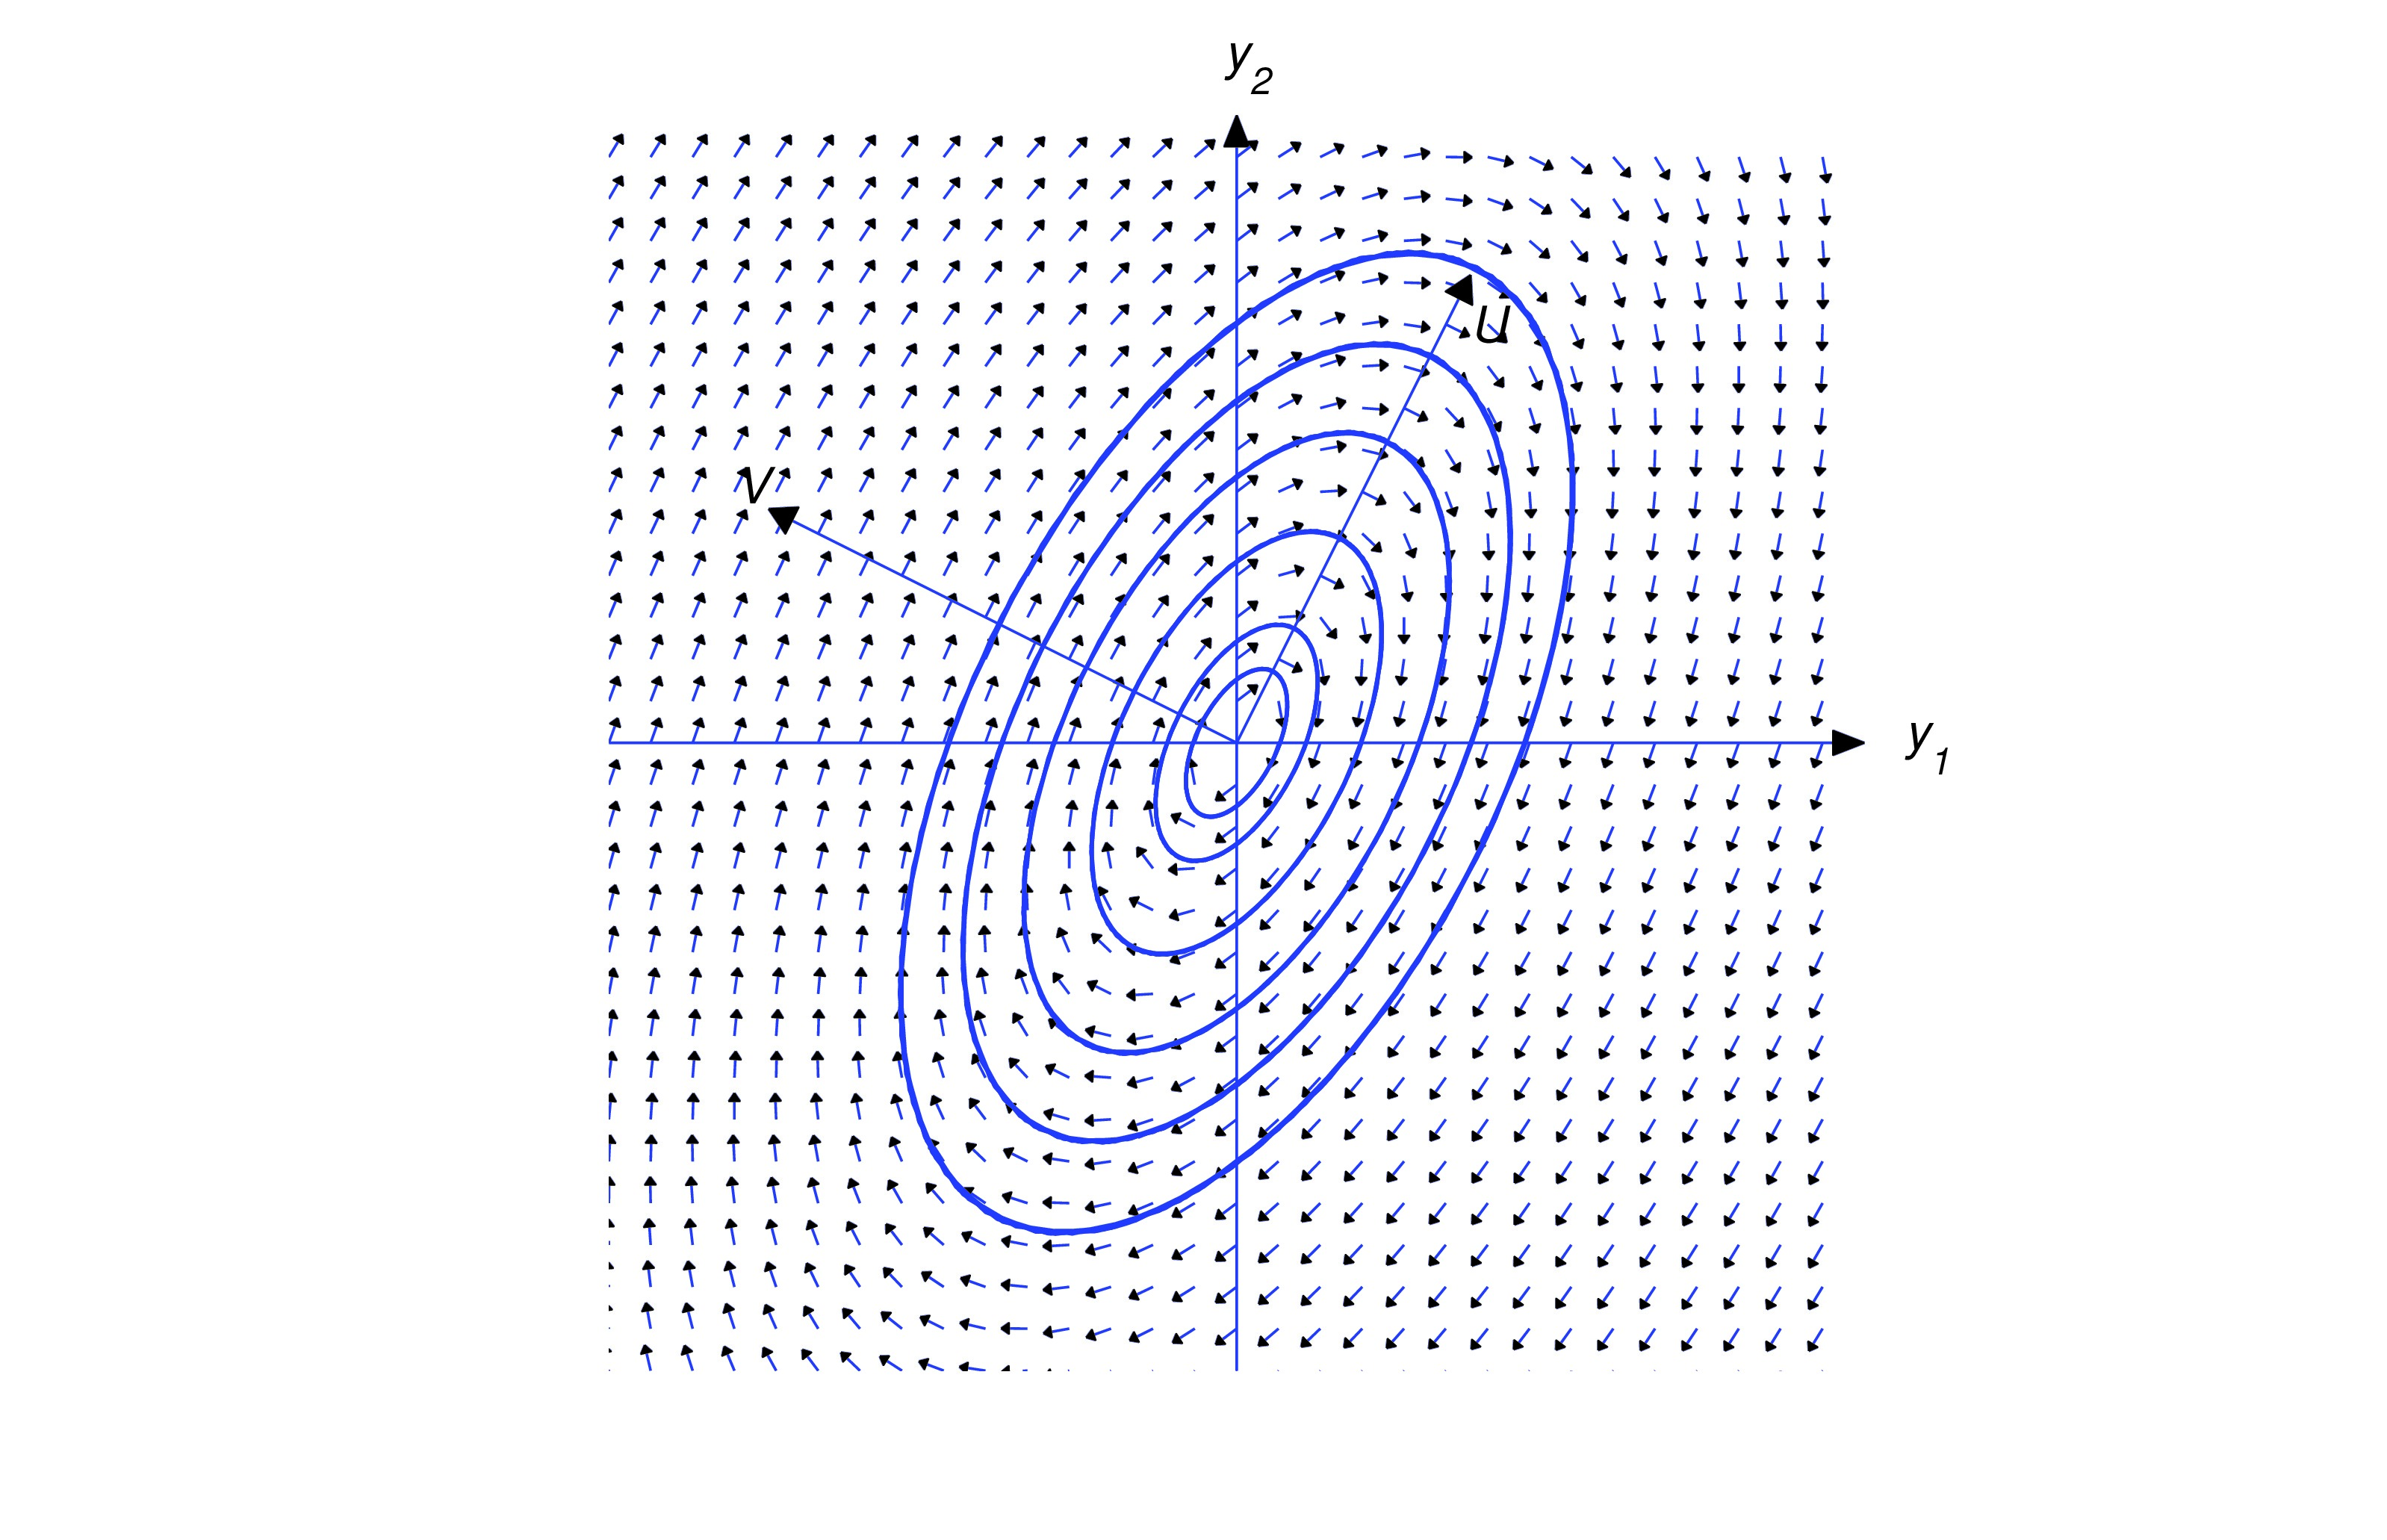
\includegraphics[height=1.5in]{fig100601.jpg} 
\end{image}

\begin{image}
 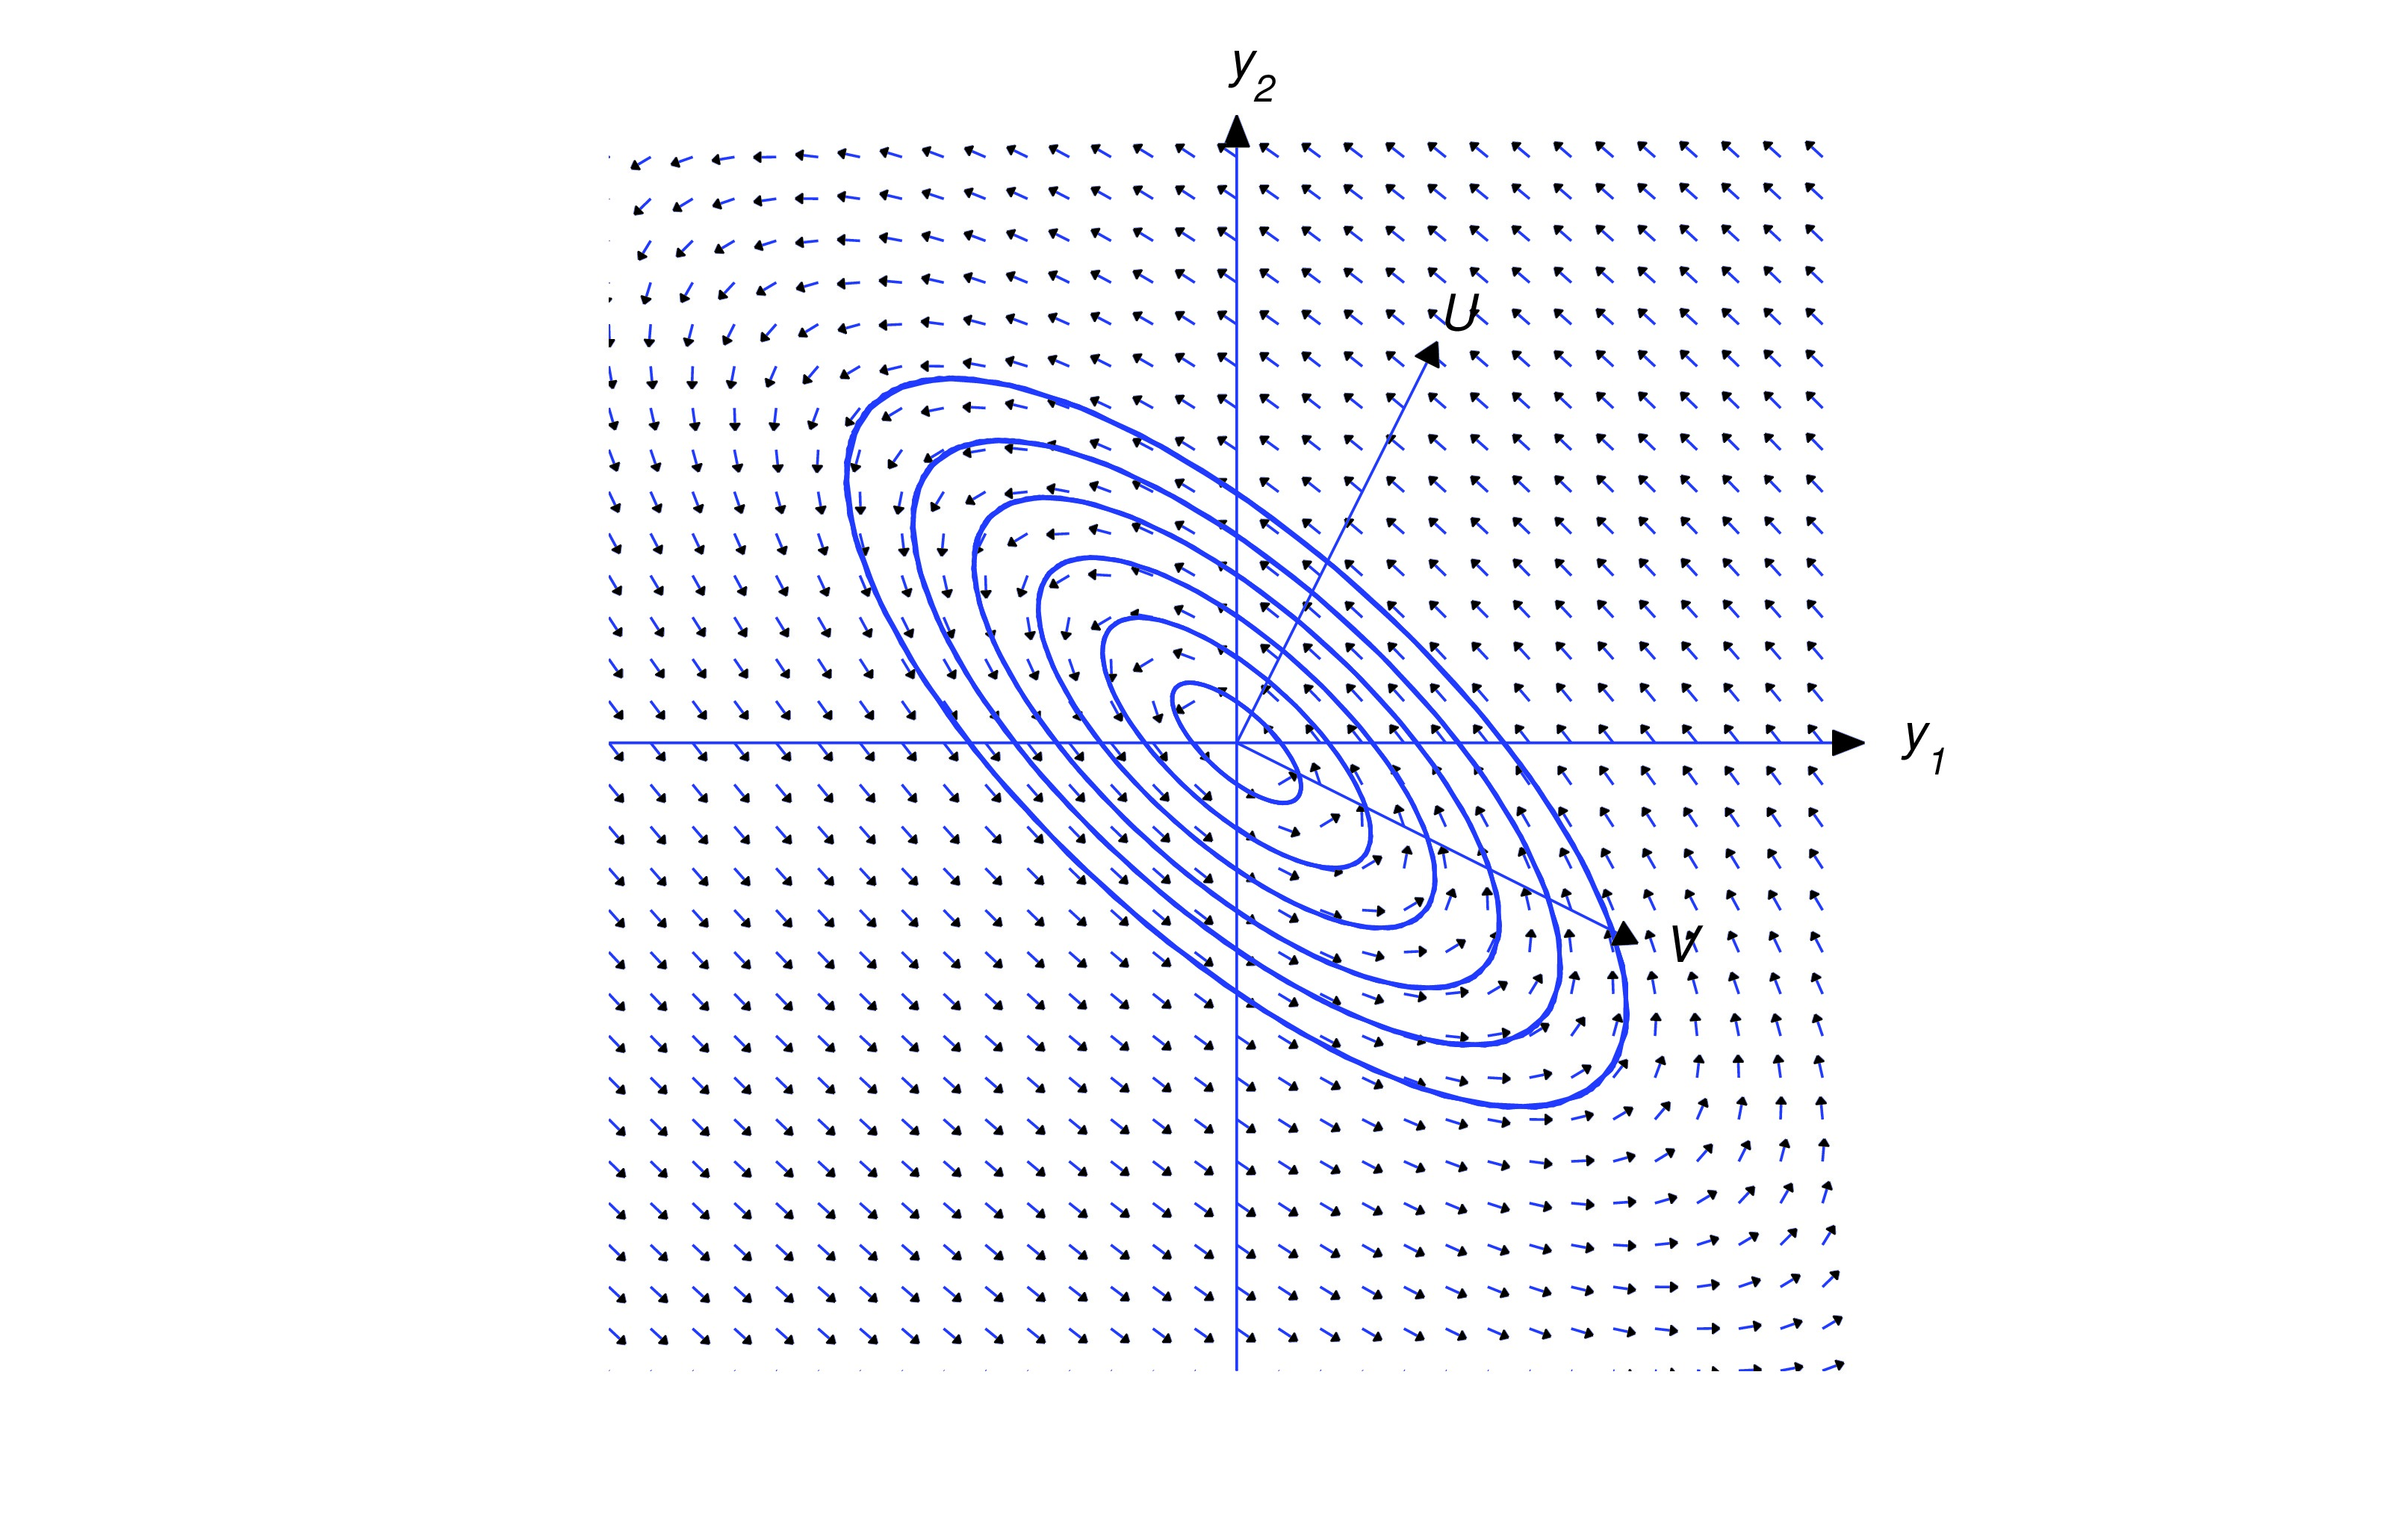
\includegraphics[height=1.5in]{fig100602.jpg} 
\end{image}


If $\alpha=0$, then any trajectory of \eqref{eq:10.6.10} is a shadow
trajectory of \eqref{eq:10.6.10};  therefore, if $\lambda$ is purely
imaginary, then the trajectories of \eqref{eq:10.6.10} are ellipses
traversed
periodically as indicated in Figures~\ref{figure:10.6.1} and
\ref{figure:10.6.2}.


If $\alpha>0$, then
$$
\lim_{t\rightarrow\infty}\norm{{\bf y}(t)}=\infty\quad\mbox{and}\quad
\lim_{t\rightarrow-\infty}{\bf y}(t)=0,
$$
so the trajectory spirals away from the origin as $t$ varies from
$-\infty$ to $\infty$. The direction of the spiral depends upon the
relative orientation of ${\bf U}$ and ${\bf V}$, as shown in
the figures below.

\begin{image}
 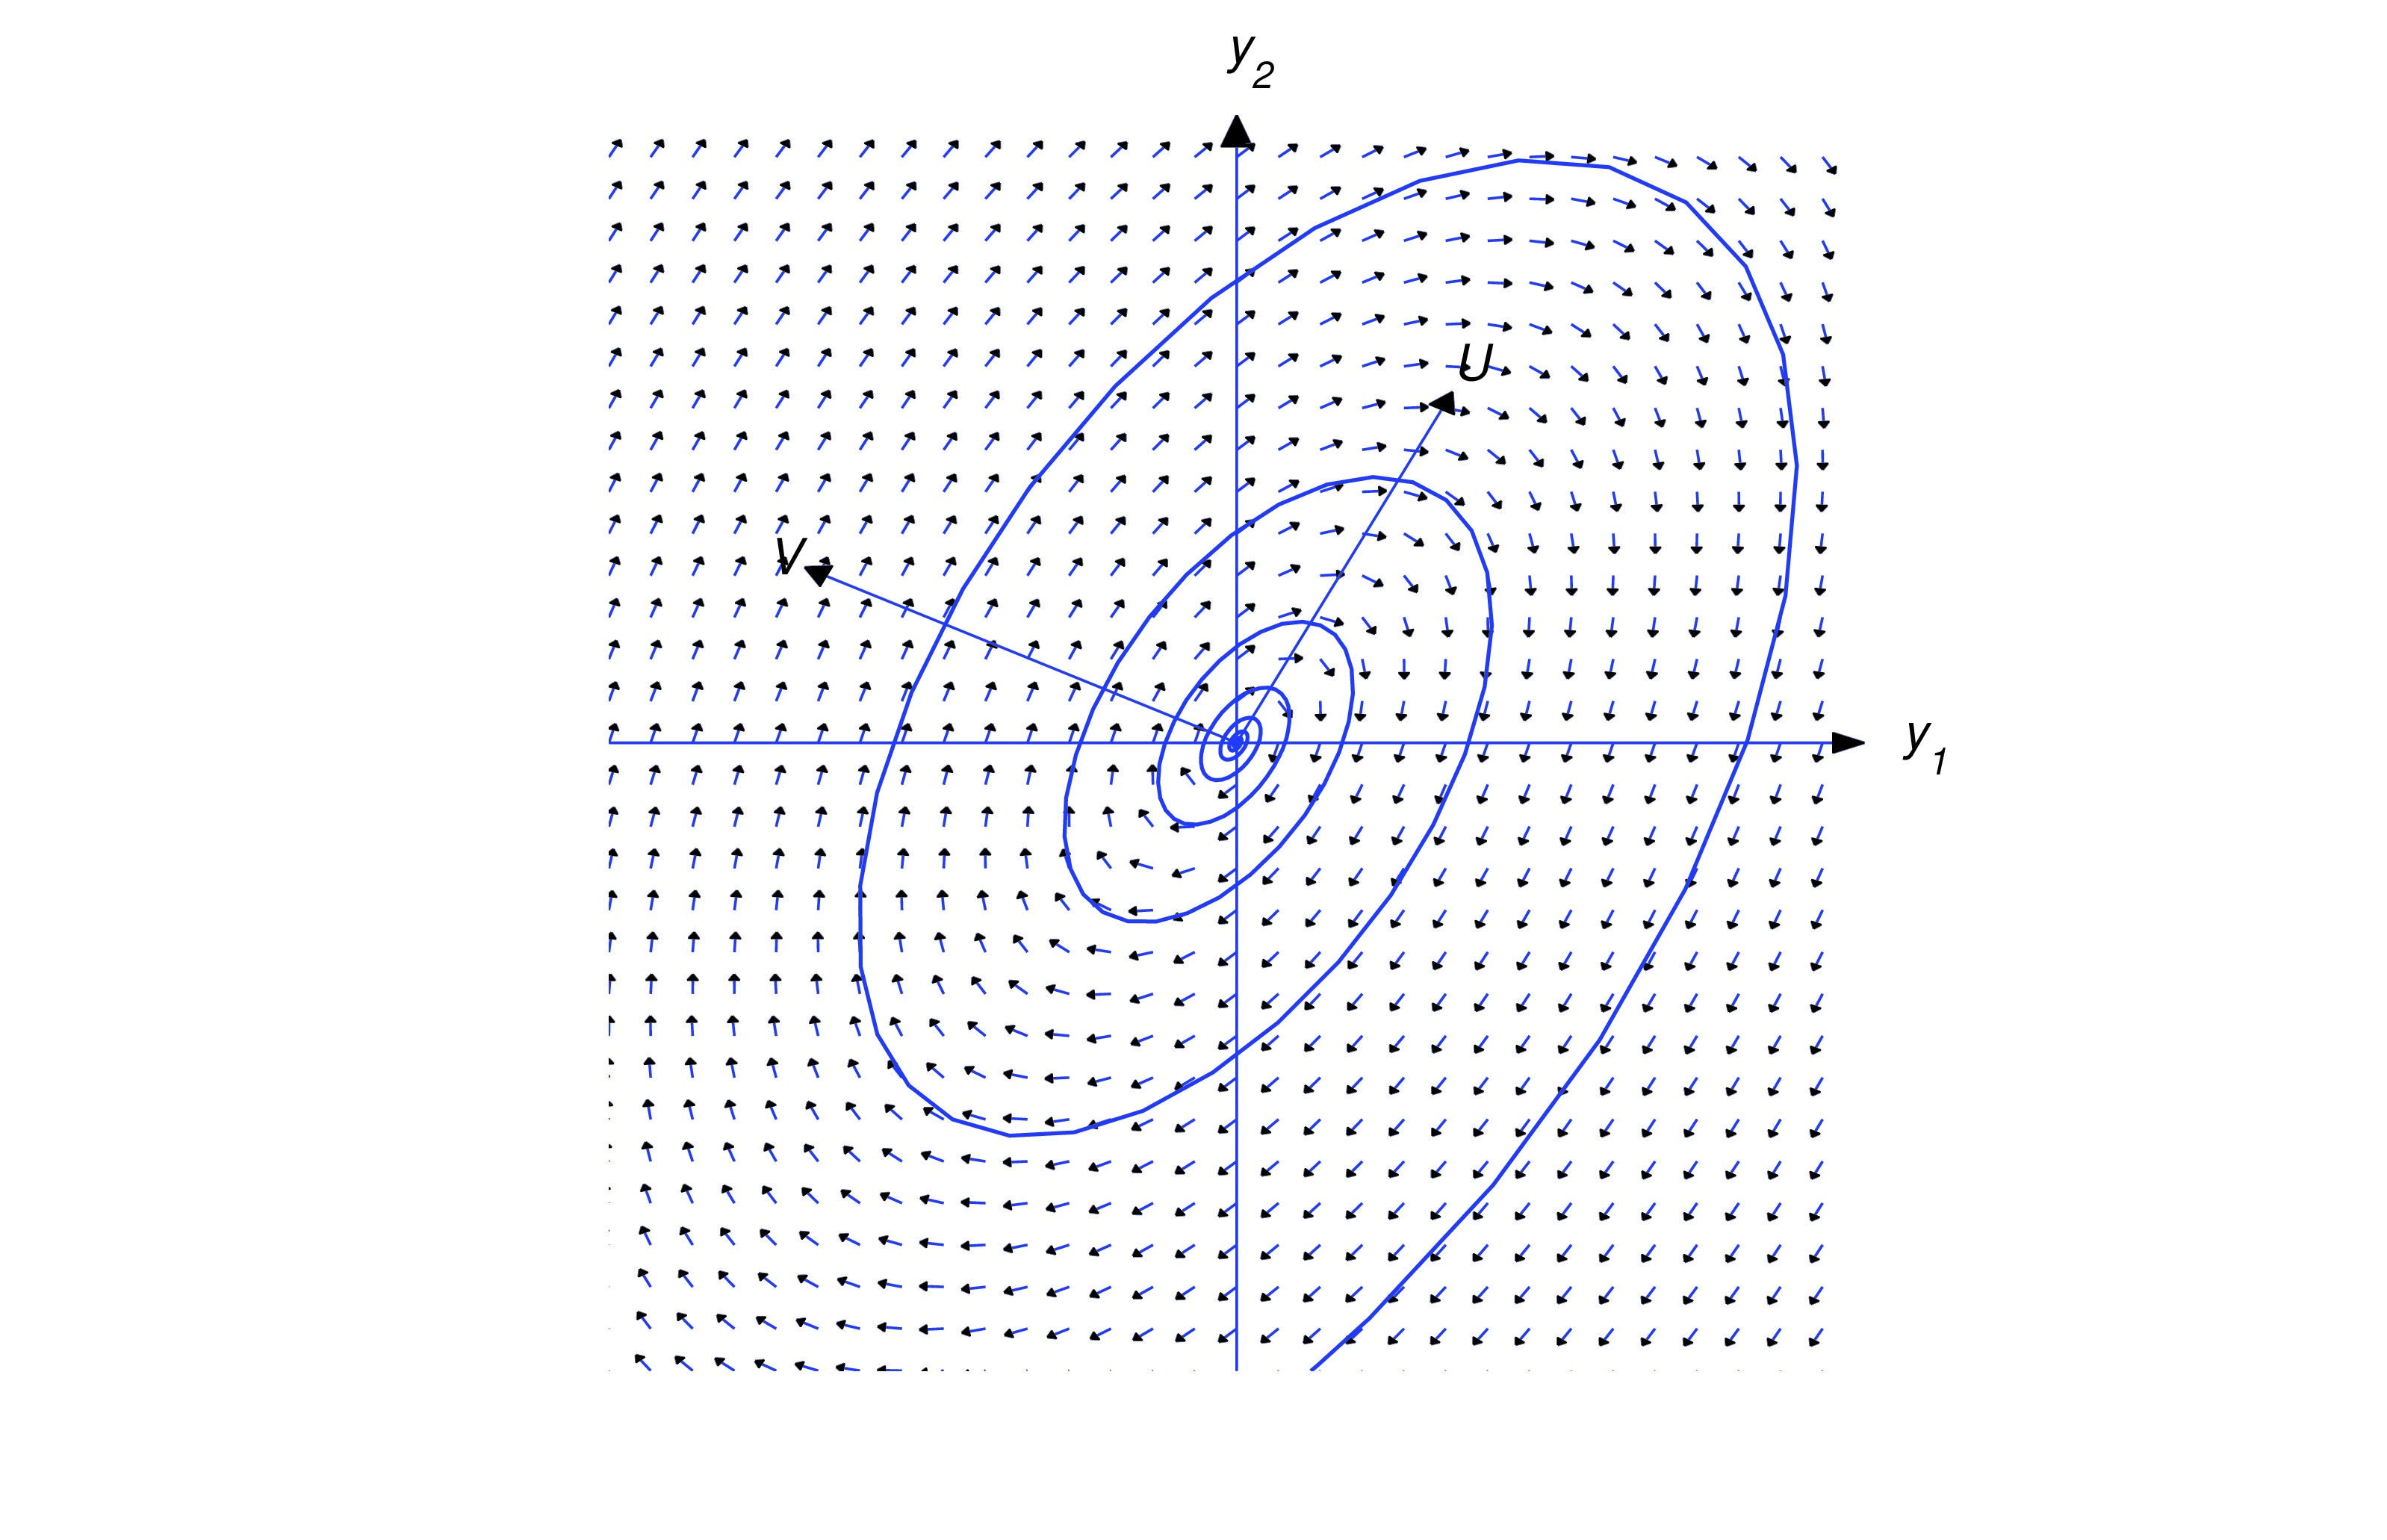
\includegraphics[height=1.5in]{fig100603.jpg} 
\end{image}

\begin{image}
 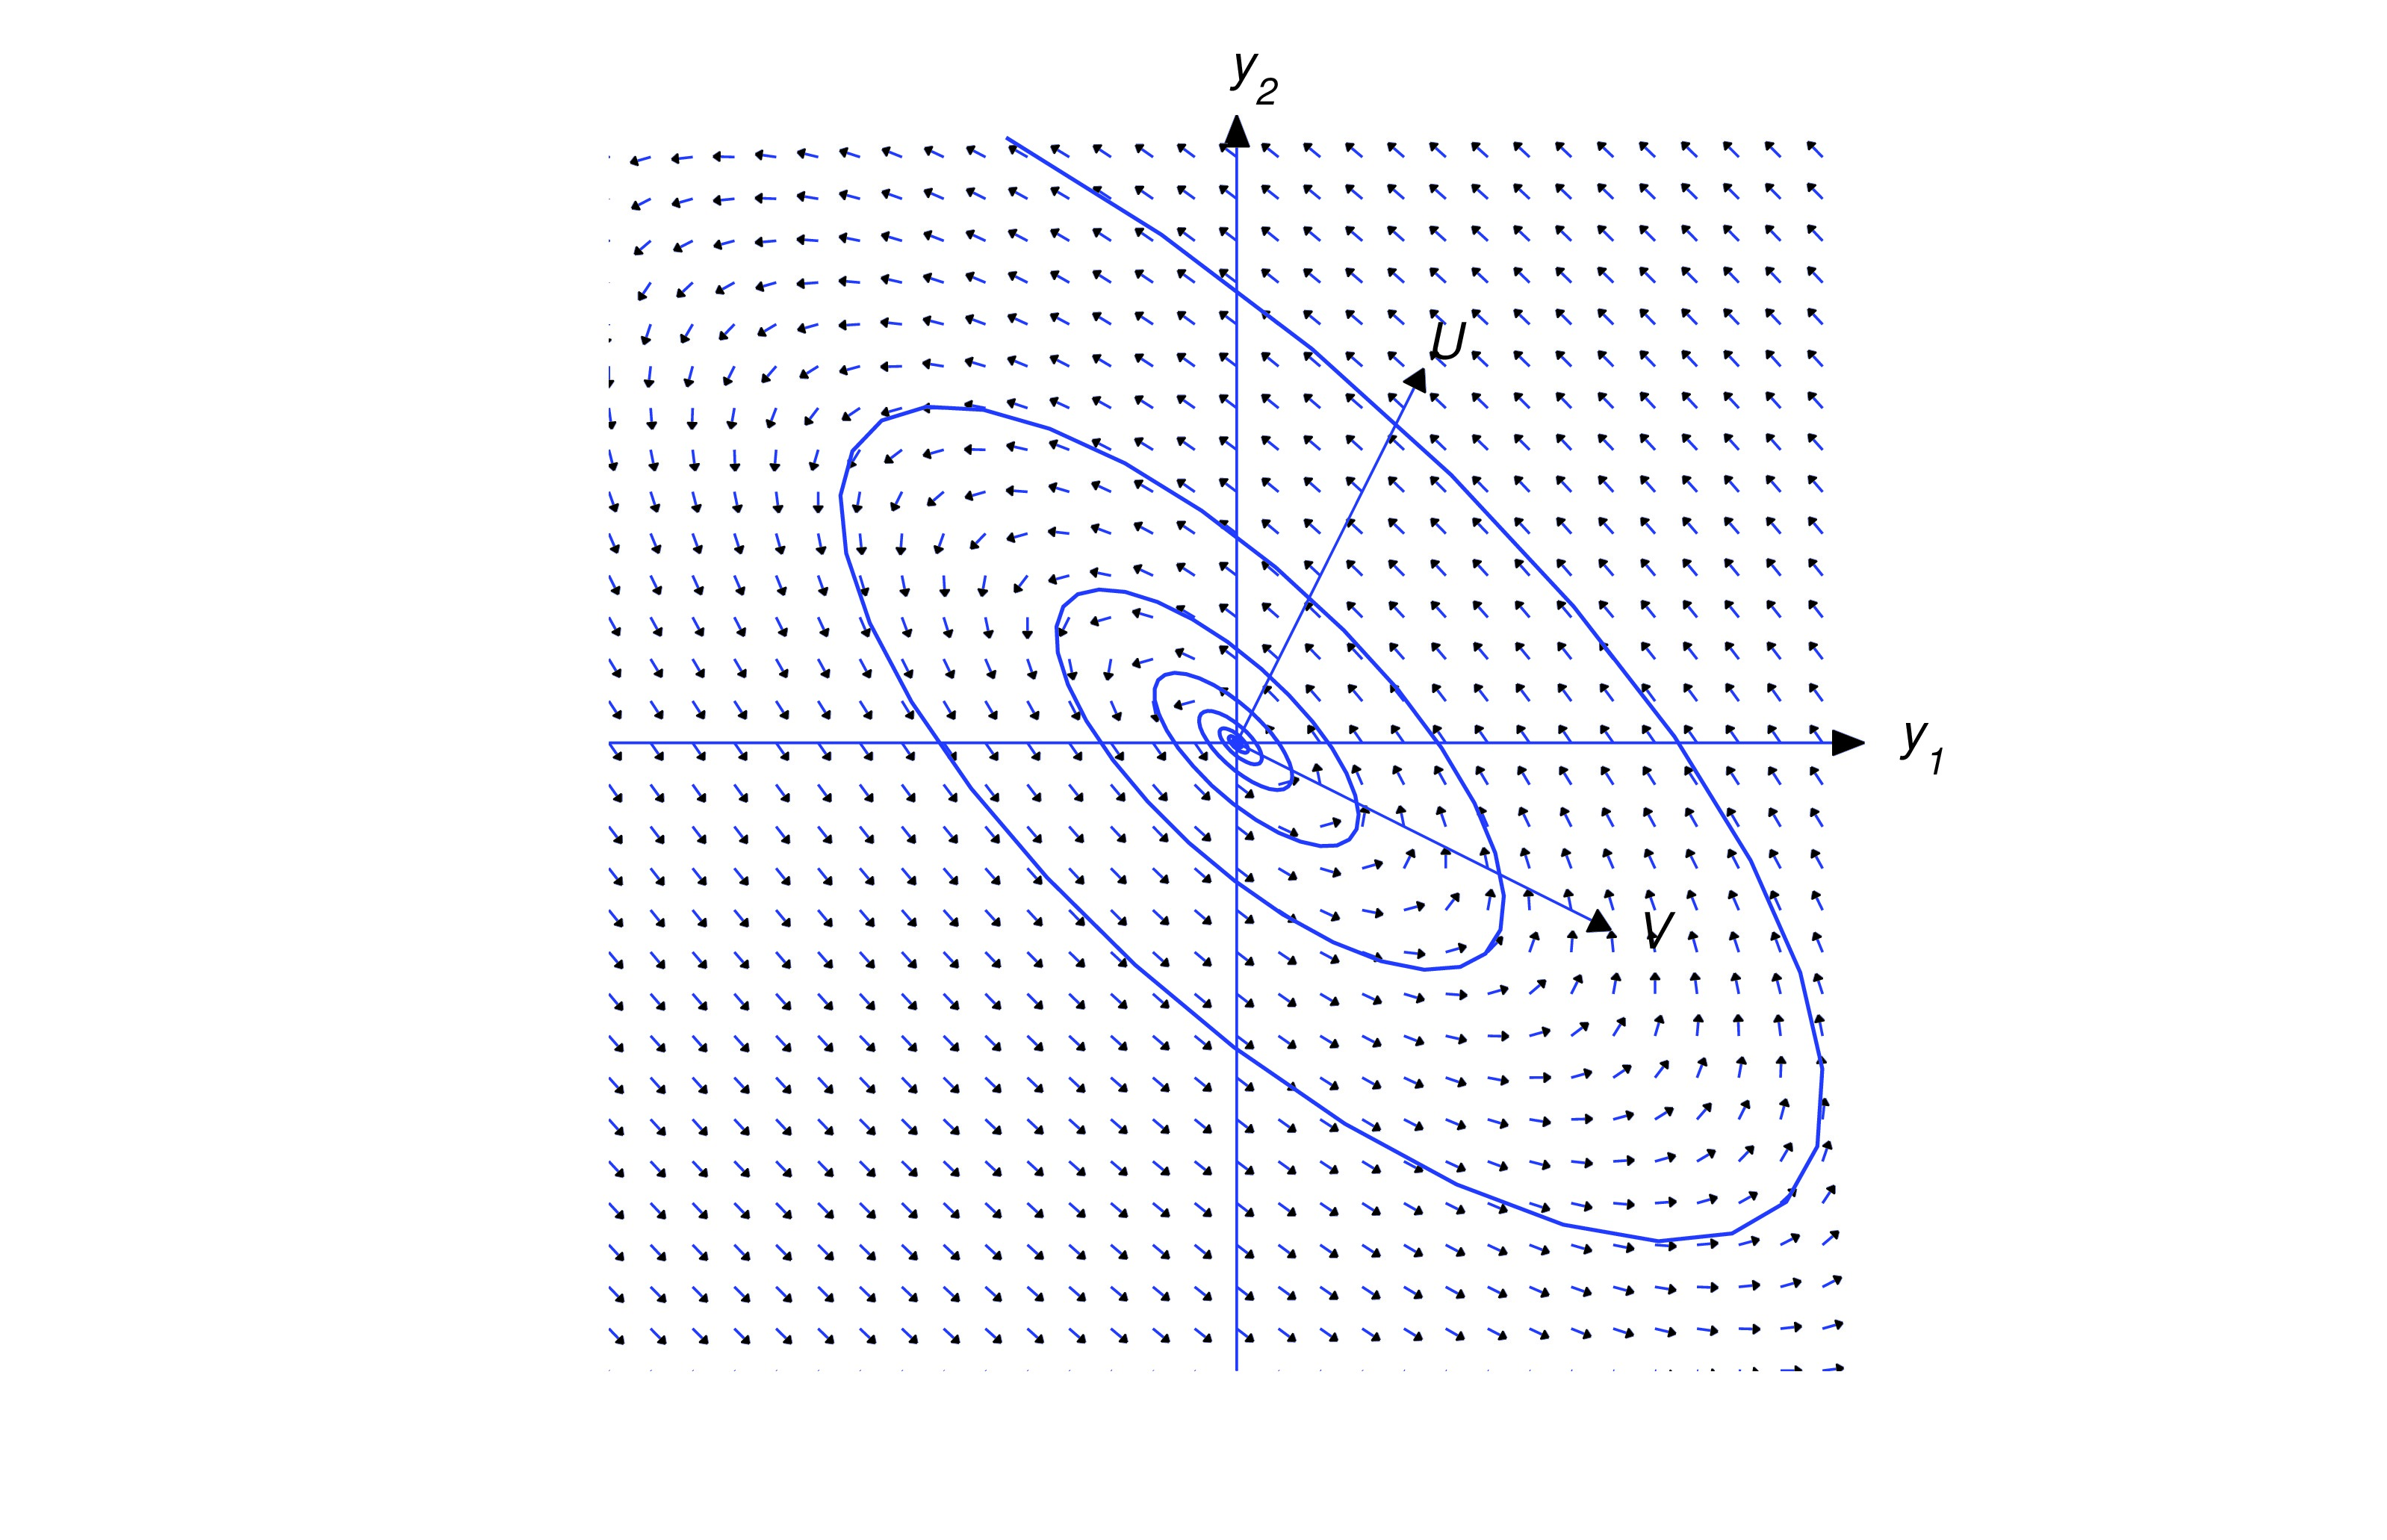
\includegraphics[height=1.5in]{fig100604.jpg} 
\end{image}


If $\alpha<0$,  then
$$
\lim_{t\rightarrow-\infty}\norm{{\bf y}(t)}=\infty\quad\mbox{and}\quad
\lim_{t\rightarrow\infty}{\bf y}(t)=0,
$$

so the trajectory spirals toward the origin as $t$ varies from
$-\infty$ to $\infty$. Again, the direction of the spiral depends upon
the relative orientation of ${\bf U}$ and ${\bf V}$, as shown in the figures below.

\begin{image}
 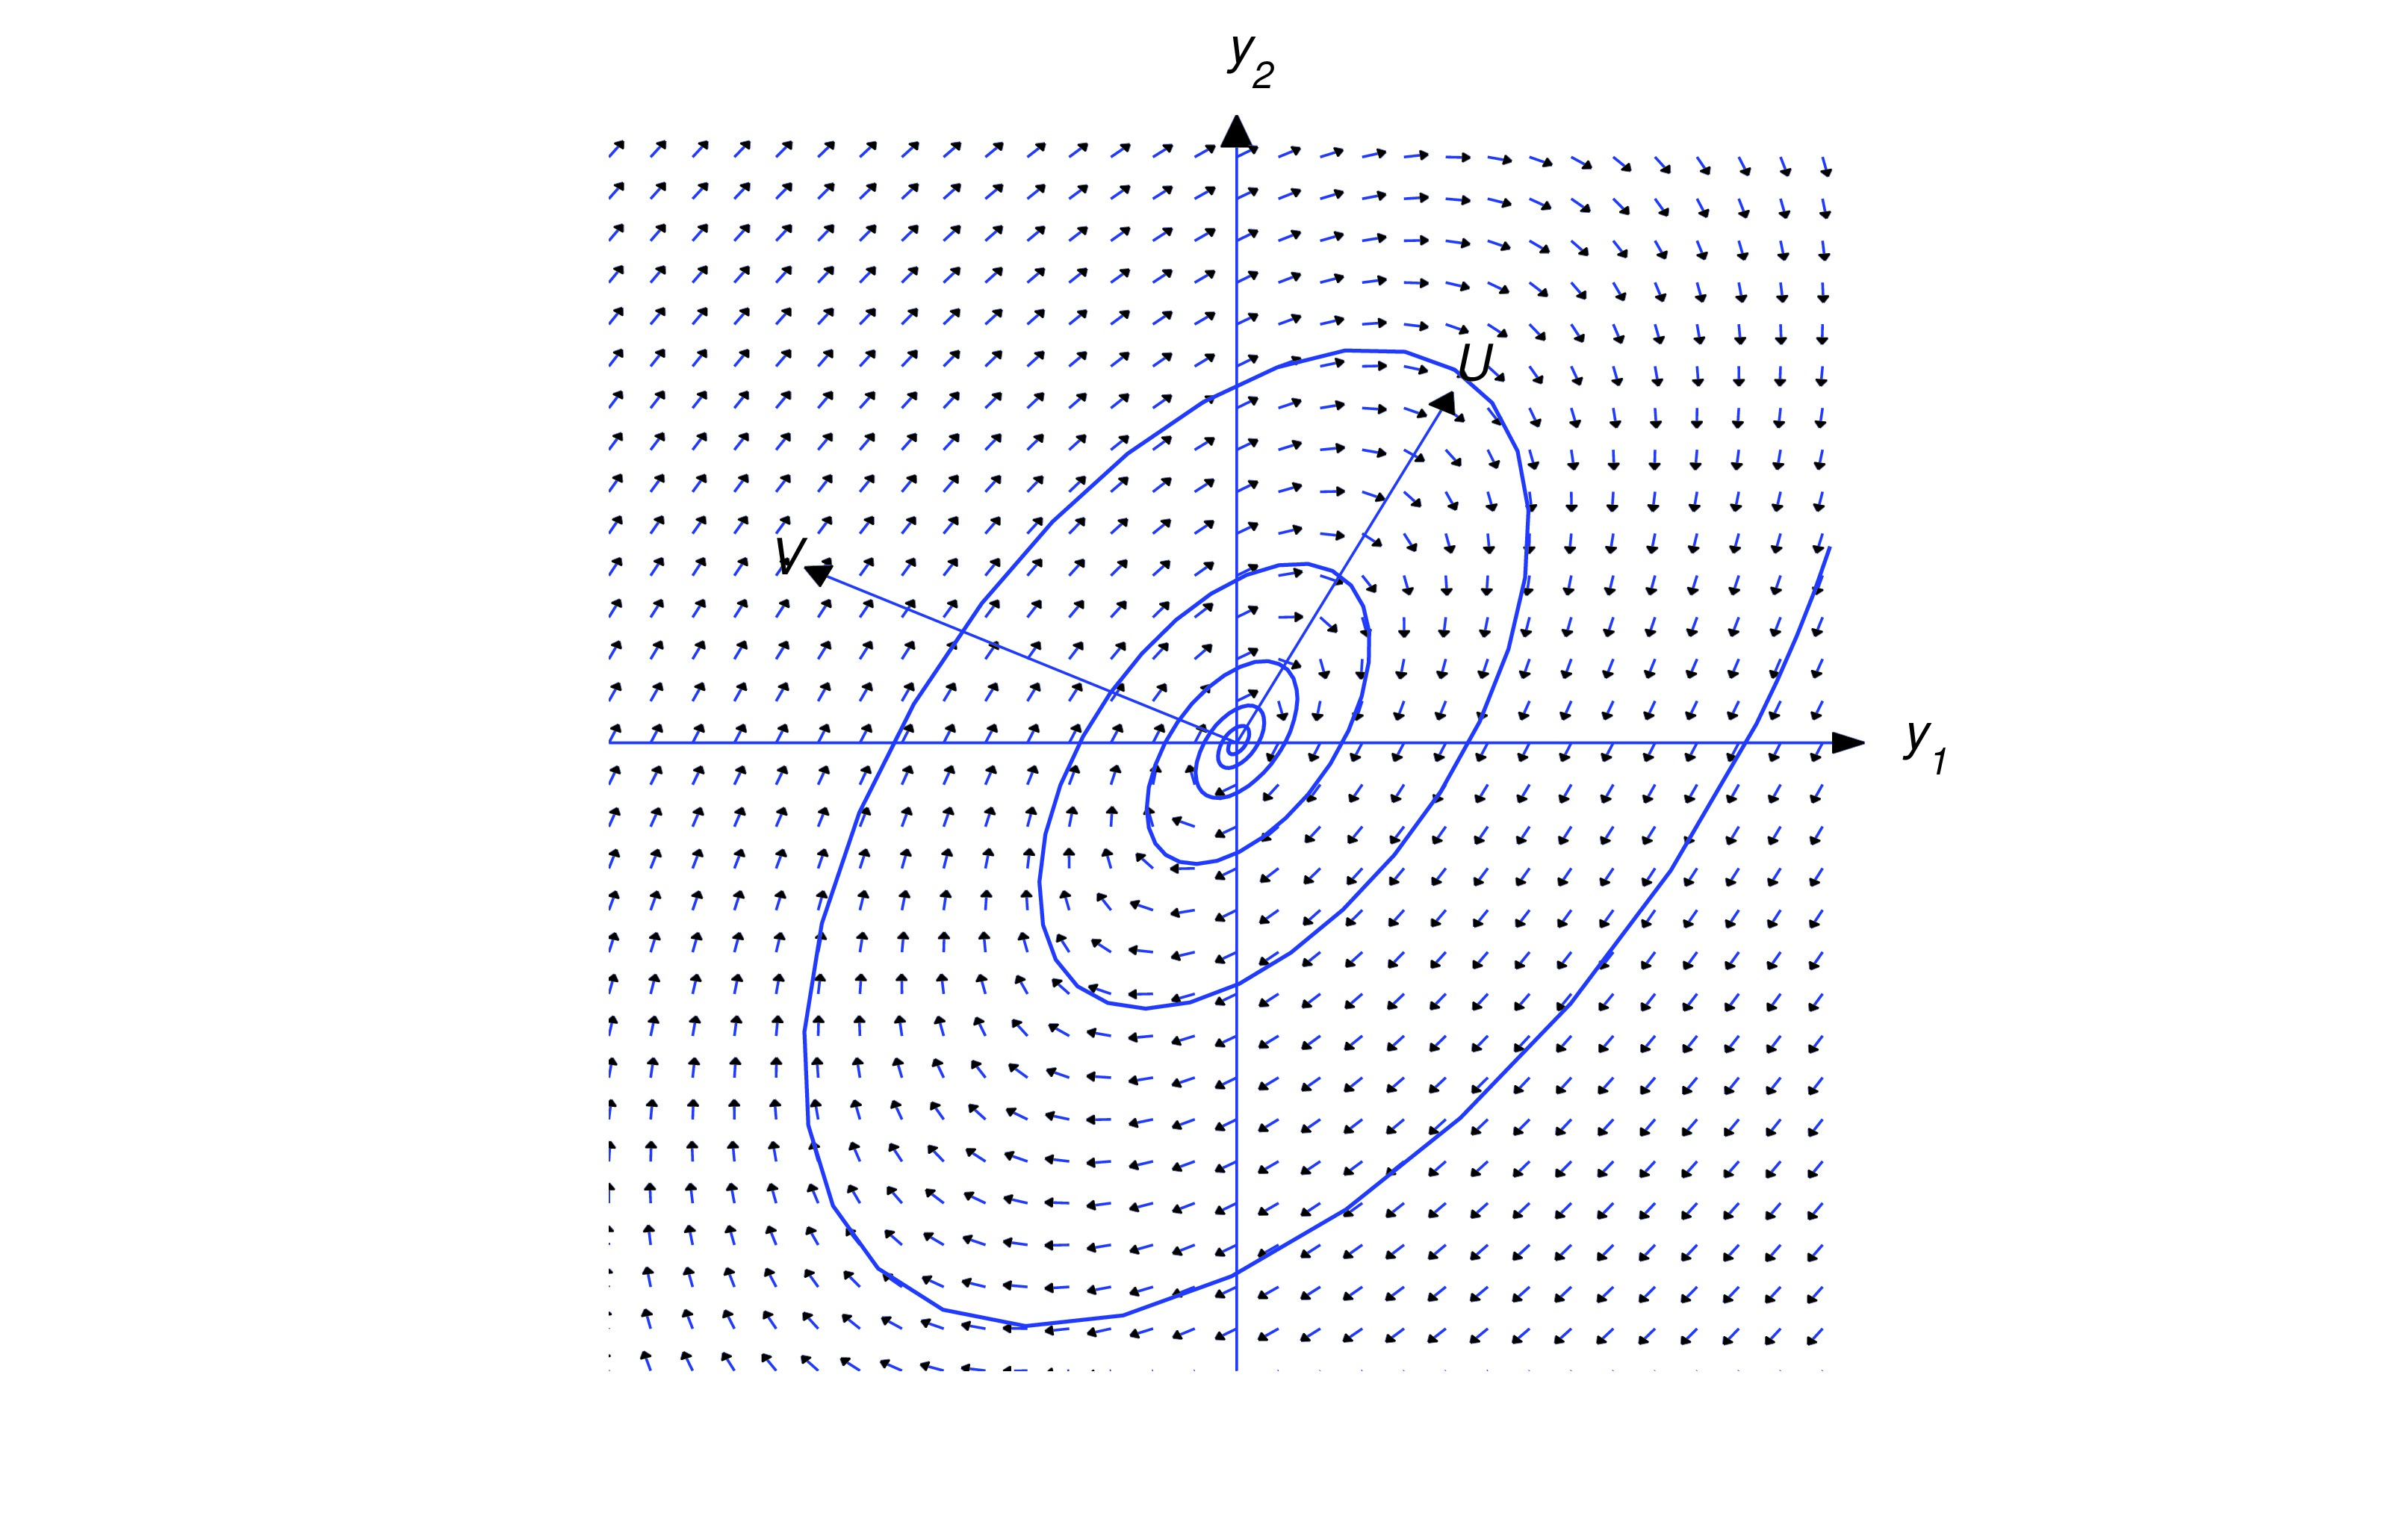
\includegraphics[height=1.5in]{fig100605.jpg} 
\end{image}

\begin{image}
 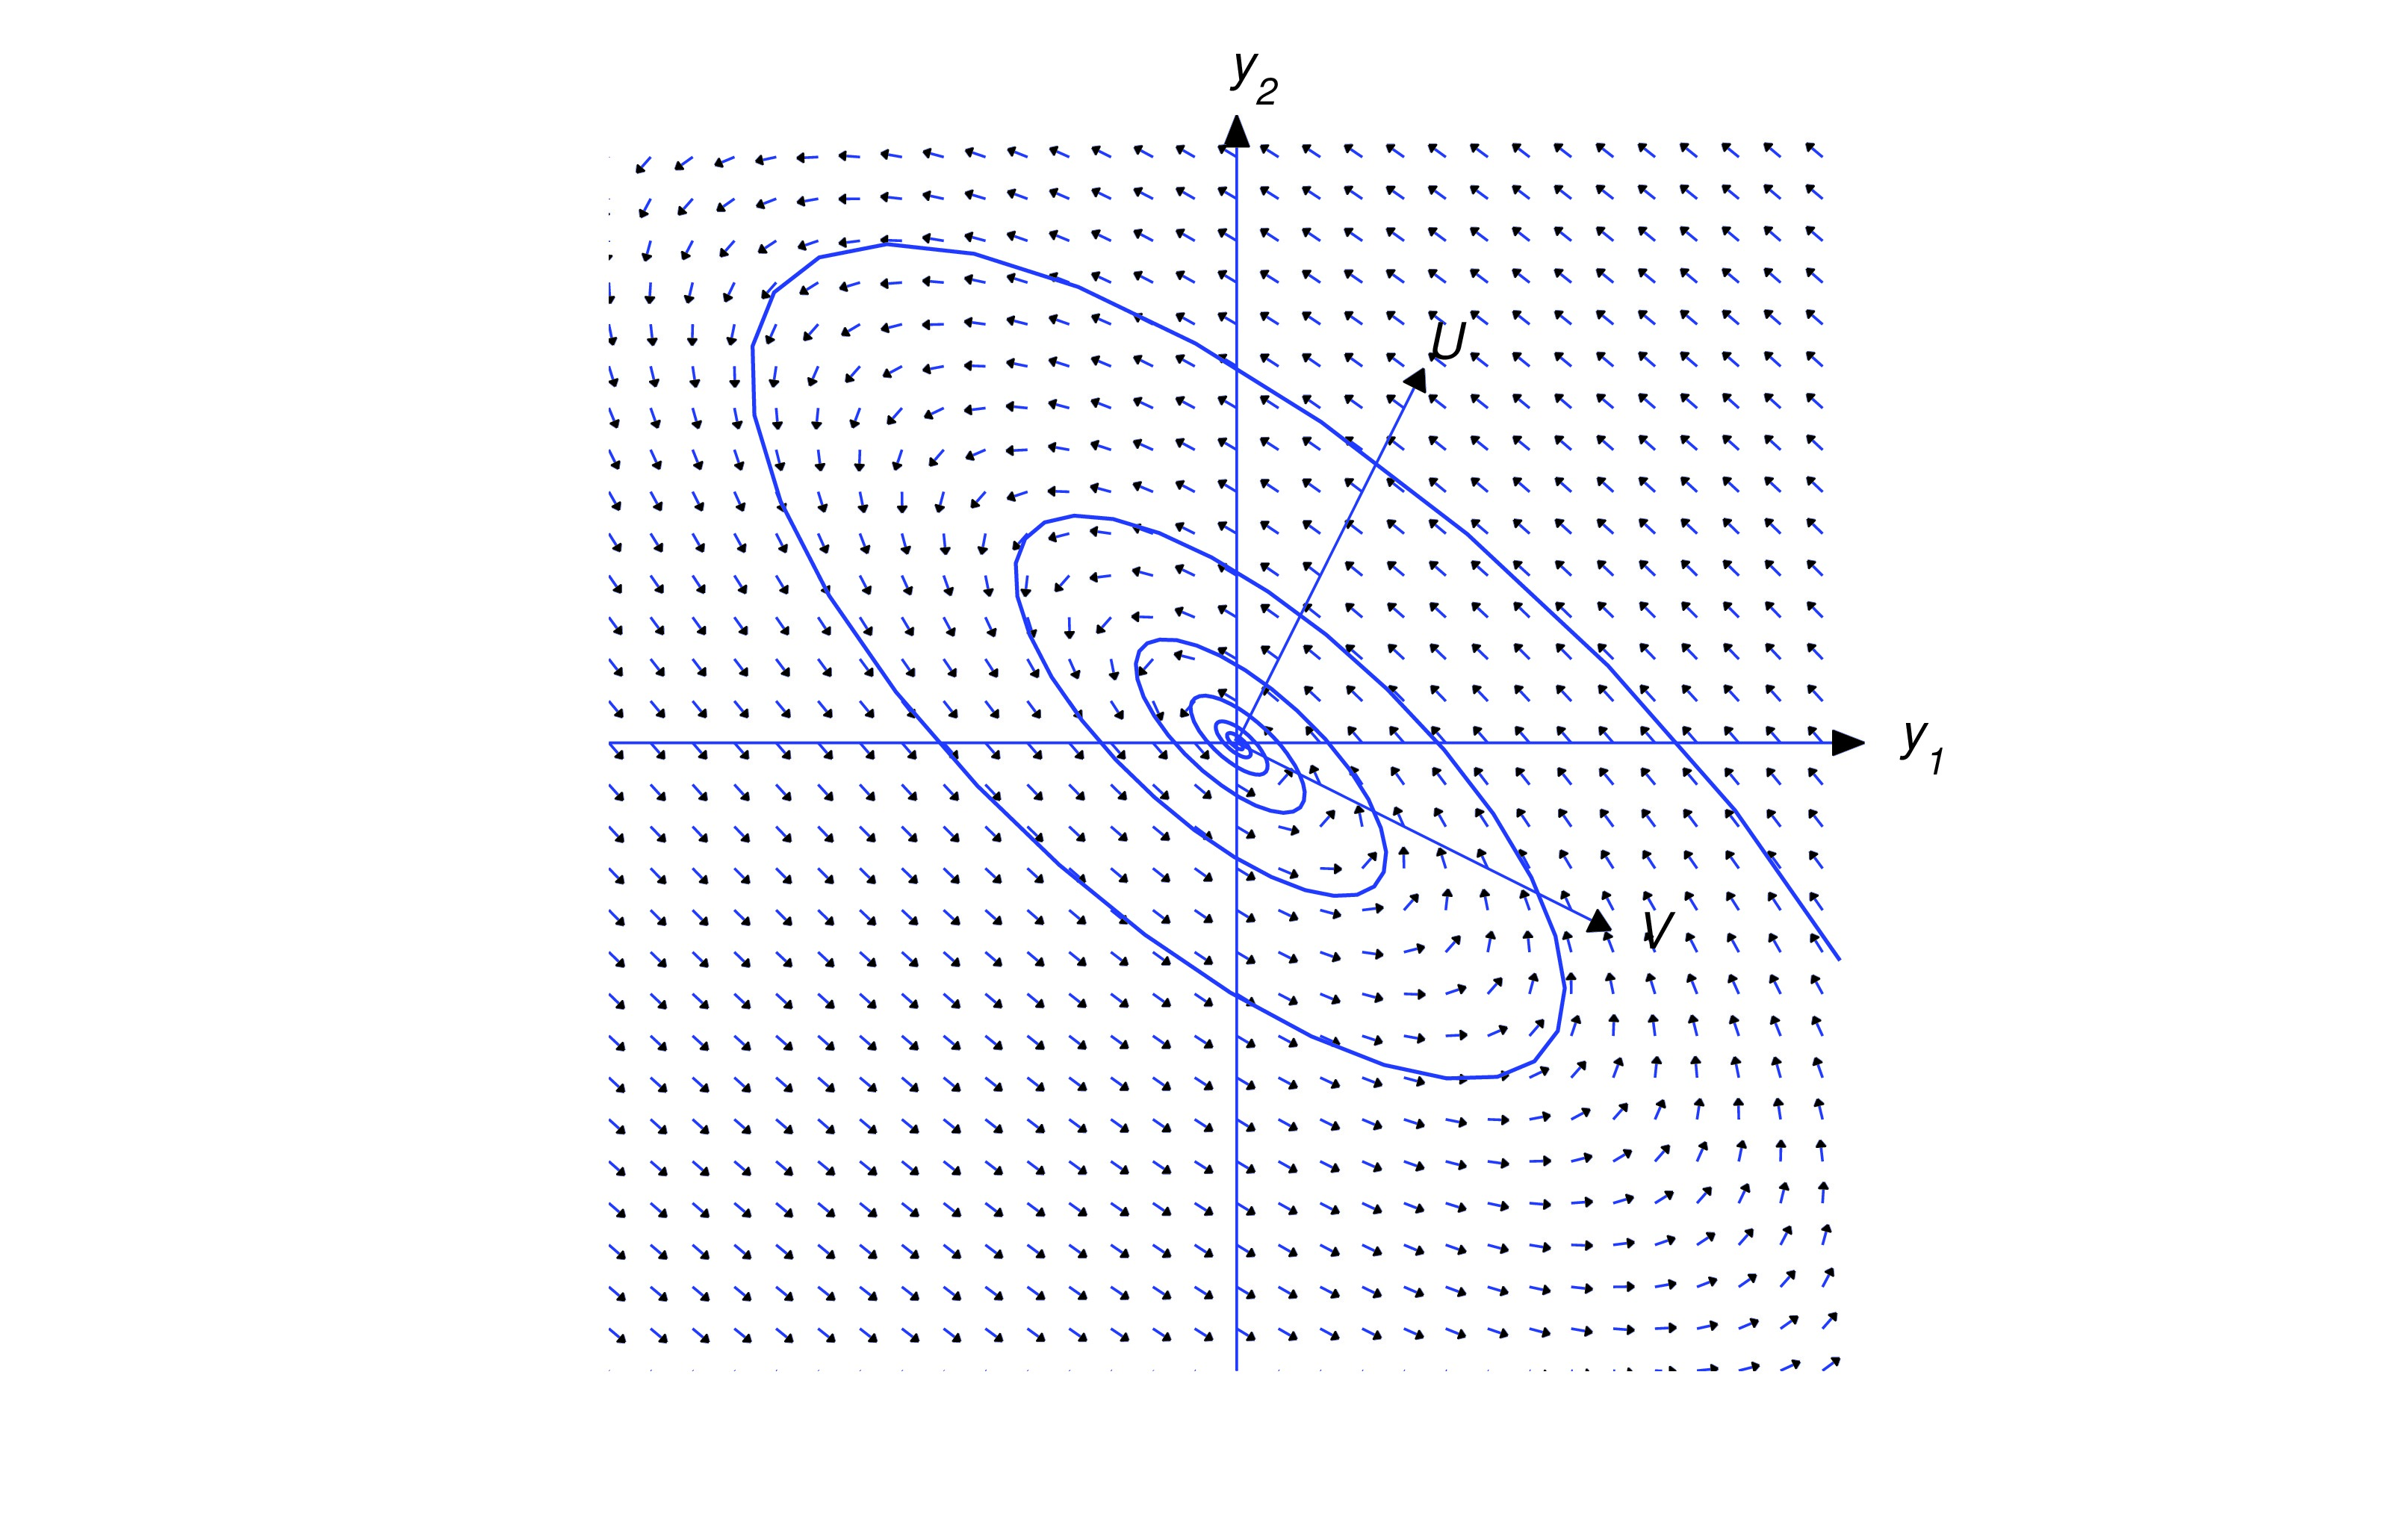
\includegraphics[height=1.5in]{fig100606.jpg} 
\end{image}


\section*{Text Source}
Trench, William F., "Elementary Differential Equations" (2013). Faculty Authored and Edited Books \& CDs. 8. (CC-BY-NC-SA)

\href{https://digitalcommons.trinity.edu/mono/8/}{https://digitalcommons.trinity.edu/mono/8/}


\end{document}